\chapter{Special Relativity: Spacetime Diagram Gallery}

This chapter collects the first locally tested spacetime diagrams for the special
relativity note.  The diagrams are intentionally simple and robust.  They are
included as TikZ inputs from the project figure directory and can later be
refined one by one.

\section{Light Cone and Interval Classification}

The light cone separates timelike, lightlike, and spacelike directions.  With
our sign convention,
\[
\Delta s^2=c^2\Delta t^2-\Delta x^2,
\]
timelike separations have \(\Delta s^2>0\), lightlike separations have
\(\Delta s^2=0\), and spacelike separations have \(\Delta s^2<0\).

\begin{figure}[h!]
  \centering
  \begin{center}
\fbox{\parbox{0.82\linewidth}{\centering Spacetime diagram temporarily disabled while TikZ sources are being corrected.}}
\end{center}

  \caption{The light cone and the classification of spacetime intervals.}
\end{figure}

\clearpage

\section{Lorentz Axes}

A Lorentz boost changes both the time and space axes.  The transformed axes tilt
toward the light cone.  Rapidity \(\varphi\) is defined by
\[
\tanh\varphi=\beta=\frac{v}{c}.
\]

\begin{figure}[h!]
  \centering
  \begin{tikzpicture}[x=1cm,y=1cm,>=Stealth]
  \draw[->] (-3.2,0) -- (3.4,0) node[right] {$x$};
  \draw[->] (0,-0.2) -- (0,3.7) node[above] {$ct$};

  \draw[dashed] (-3,-3) -- (3,3);
  \draw[dashed] (-3,3) -- (3,-3);

  \draw[very thick,->] (-2.8,-1.5) -- (3.0,1.65) node[right] {$x'$};
  \draw[very thick,->] (-1.5,-2.8) -- (1.85,3.45) node[above] {$ct'$};

  \fill (0,0) circle (1.3pt) node[below left] {$O$};
  \node[align=left,anchor=west] at (-3.0,3.2) {$\tanh\varphi=\beta=v/c$\\axes tilt toward the light cone};
\end{tikzpicture}

  \caption{Lorentz-transformed axes in a spacetime diagram.}
\end{figure}

\clearpage

\section{Relativity of Simultaneity}

The transformation
\[
\Delta t'=\gamma\left(\Delta t-\frac{v\Delta x}{c^2}\right)
\]
shows that events simultaneous in one frame need not be simultaneous in another
frame.  In spacetime geometry, this is represented by different simultaneity
slices.

\begin{figure}[h!]
  \centering
  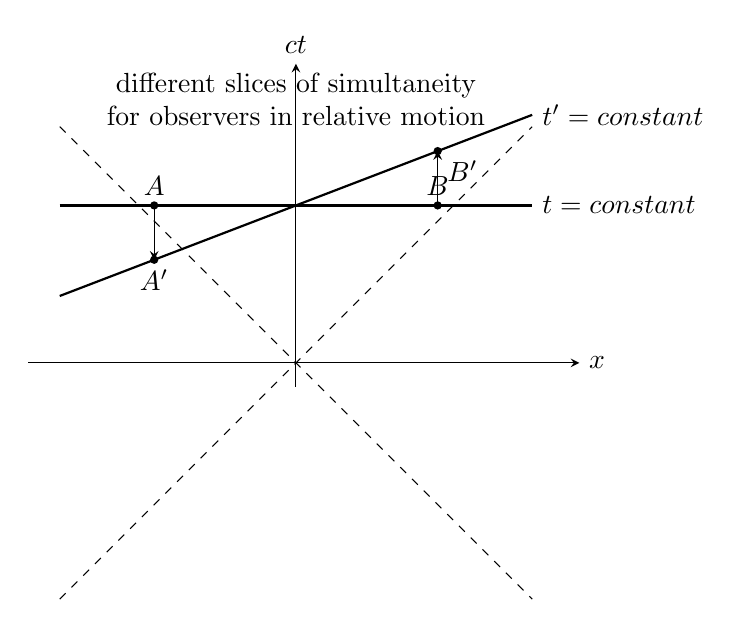
\begin{tikzpicture}[x=1cm,y=1cm,>=stealth]
    \draw[->] (-3.4,0) -- (3.6,0) node[right] {\(x\)};
    \draw[->] (0,-0.3) -- (0,3.8) node[above] {\(ct\)};

    \draw[dashed] (-3,-3) -- (3,3);
    \draw[dashed] (-3,3) -- (3,-3);

    % laboratory simultaneity
    \draw[thick] (-3,2.0) -- (3,2.0) node[right] {\(t=\text{constant}\)};
    \fill (-1.8,2.0) circle (1.5pt) node[above] {\(A\)};
    \fill (1.8,2.0) circle (1.5pt) node[above] {\(B\)};

    % moving-frame simultaneity, ct' constant: ct - beta x = const
    \draw[thick] (-3,0.85) -- (3,3.15) node[right] {\(t'=\text{constant}\)};
    \fill (-1.8,1.31) circle (1.5pt) node[below] {\(A'\)};
    \fill (1.8,2.69) circle (1.5pt) node[below right] {\(B'\)};

    \draw[->] (-1.8,2.0) -- (-1.8,1.31);
    \draw[->] (1.8,2.0) -- (1.8,2.69);
    \node[align=center] at (0,3.35) {different slices of simultaneity\\for observers in relative motion};
\end{tikzpicture}

  \caption{Two different simultaneity slices for observers in relative motion.}
\end{figure}

\clearpage

\section{Time Dilation}

Two ticks of one moving clock lie on the same worldline.  The proper time is the
invariant time measured along that clock's worldline:
\[
(c\Delta\tau)^2=(c\Delta t)^2-(\Delta x)^2.
\]
This gives
\[
\Delta t=\gamma\Delta\tau.
\]

\begin{figure}[h!]
  \centering
  \begin{tikzpicture}[x=1cm,y=1cm,>=Stealth]
  \draw[->] (-0.5,0) -- (5.4,0) node[right] {$x$};
  \draw[->] (0,-0.2) -- (0,4.6) node[above] {$ct$};

  \draw[thick] (0.9,0.2) -- (0.9,4.0);
  \fill (0.9,1.0) circle (1.4pt) node[left] {tick 1};
  \fill (0.9,3.2) circle (1.4pt) node[left] {tick 2};

  \draw[thick] (2.2,0.4) -- (4.1,4.2);
  \fill (2.55,1.1) circle (1.4pt) node[right] {tick 1};
  \fill (3.55,3.1) circle (1.4pt) node[right] {tick 2};

  \node[align=left,anchor=west] at (1.3,4.15)
    {Proper time is measured\\along one clock's worldline:\\$(c\Delta\tau)^2=(c\Delta t)^2-(\Delta x)^2$};
\end{tikzpicture}

  \caption{Time dilation represented by two ticks on a clock worldline.}
\end{figure}

\clearpage

\section{Length Contraction}

A length measurement compares the positions of both endpoints at the same time
in the measuring frame.  The resulting contracted length is
\[
L=\frac{L_0}{\gamma}.
\]

\begin{figure}[h!]
  \centering
  \begin{tikzpicture}[x=1cm,y=1cm,>=Stealth]
  \draw[->] (-0.3,0) -- (5.8,0) node[right] {$x$};
  \draw[->] (0,-0.2) -- (0,4.5) node[above] {$ct$};

  \draw[thick] (0.8,0.2) -- (2.2,4.2) node[above] {rear end};
  \draw[thick] (3.1,0.2) -- (4.5,4.2) node[above] {front end};

  \draw[very thick] (1.43,2.0) -- (3.73,2.0);
  \fill (1.43,2.0) circle (1.4pt);
  \fill (3.73,2.0) circle (1.4pt);
  \node[above] at (2.58,2.05) {$L=L_0/\gamma$};

  \draw[dashed] (1.02,0.82) -- (3.32,2.12);
  \node[below right] at (2.55,1.55) {$t'=\mathrm{const}$};
\end{tikzpicture}

  \caption{Length contraction from simultaneous endpoint measurements.}
\end{figure}

\clearpage

\section{Muon Lifetime Geometry}

Muon survival can be described in two equivalent ways.  In the Earth frame, the
muon's lifetime is dilated.  In the muon frame, the atmospheric distance is
length-contracted.  Both descriptions refer to the same pair of physical events.

\begin{figure}[h!]
  \centering
  \begin{tikzpicture}[x=1cm,y=1cm,>=Stealth]
  \draw[->] (-0.2,0) -- (6.2,0) node[right] {distance};
  \draw[->] (0,-0.2) -- (0,4.8) node[above] {time};

  \draw[thick] (0.7,4.1) -- (5.4,0.7);
  \fill (0.7,4.1) circle (1.4pt) node[above right] {created};
  \fill (5.4,0.7) circle (1.4pt) node[below right] {detected};

  \draw[dashed] (0.7,0.7) -- (5.4,0.7);
  \draw[dashed] (0.7,0.7) -- (0.7,4.1);

  \node[align=left,anchor=west] at (1.0,2.7)
    {Earth frame: lifetime dilates.\\Muon frame: atmosphere contracts.};
\end{tikzpicture}

  \caption{Muon survival described by time dilation or length contraction.}
\end{figure}
